\section{Energy Consumption Analysis}
\label{sec:control}

\subsection{Occupancy Monitoring and Data analysis}

Occupants' mobility and behaviour in a building are important parameters in controlling energy consumption.  Occupancy data collected  must be analyzed first before serving as input to an energy controller. This data is initially collected by a Microsoft Kinect for Windows (K4W) sensor by our developed Occupancy-Counter software.


\subsection{Optimal control and planning}
The simplest control in an HVAC system is the cycling or OFF/ON control to meet partial load conditions. If the building only needs half of the energy that the system is designed to deliver, the system runs for some period, turns off for the next period, and then cycles on again. As the building load increases, the system runs longer and its off period is shorter. An alternative method of control under part-load conditions is staging. When conditions call for half the design capacity, only two units operate. At 60\% load, two units are base-loaded (run continuously), and a third unit swings (is either cycled or modulated) as needed. If it is assumed that Units 1 and 2 are base-loaded, and Unit 3 has just cycled on. The three ways of saving energy as mention in \cite{fnd} are then: Turn it OFF, Turn it DOWN or Turn it IN. The first refers to the first control method of cycling while the second refers to the staging usage, where part of the units are put on cycling and the other parts are operated with a low set-point. The last one refers to replacing or changing the air conditioning unit with a new one for more efficiency.

On the other hand, there are many other factors that play important roles in controlling air conditioning systems. These factors are:
\textbf{ The person thermal comfort:} There are different factors that influence thermal comfort including: clothing (level of cloths), activity level(human body release heats), air flow( direction of air), air temperature ( the level of cooling), and expectations( which vary from one person to another).
\textbf{ Space Size:} The small room size is different than a big one. The number of pieces of operating equipment is important since it releases some heat. To go on real-time controlling, it might consider the combined number of sensors that can include
\textbf{Space Design :}the number of windows and doors in the building. Windows bring the heat load from the sun and doors release the air out of the cooling space. More factors can be found in \cite{fnd}


These automated control systems require full coverage of all above factors in order to say that air conditioning systems have been controlled efficiently. A system has been created that can display and show the occupancy time. A dynamic control method can be modelled from this system. As mentioned earlier, a Markov chain was used to create a matrix that predicted the future of moving from one state to another.  It is possible to benefit from these transition matrices by merging them to some controlling functions.It is possible to set the thermostat point to a certain point matching a certain event that occurs on the monitoring systems. Saying that, the probability to move from $state= (E,E,E,E)$ to $state=(E,A,E,E)$ after a hour will manage to open the air conditioning system at zone2 which represents the average occupancy one hour later. The remaining zones will maintain the temperature depending on the status information. This can be easily read from the display colours. The controller logic will work as a robotic command generator depending on the events created from our occupancy monitoring system. The main controller is programmable to keep a log for all states and zone conditions of the building. When some states occur they will generate new events which imply creating a control command to resolve the event issues.


\subsection{Simulation approach}

A net zero energy office building is simulated using the 'eQuest' building energy software adhering to Masdar Energy Design Guidelines (MEDG)based on the American Society of Heating, Refrigerating and Air-Conditioning (ASHRAE) 90.1. The office building is a two story building with a total floor area of $232m^2$. Each floor is divided into four office space with a floor area of $40m^2$ each. Windows are placed on the north, east and west walls of the building with overhangs having a projection factor (overhang depth/window height) of $0.6$. Two doors are placed on the north and east sides of the building. Windows and doors are not specified on the south wall to minimize heat gain through radiation. The window to gross wall area is kept at 29\%. The cooling system specified is a packaged direct expansion unit which delivers cooling through ducting.
The office space is designed for a total occupancy of 60 persons with $4.6 m^2$ per person. The air requirements are specified according to ASHRAE standard 62.1. The office space is specified as 20cfm/person(Indoor air quality method 2011) each.

\begin{figure}[!ht]
  \centering
 	  	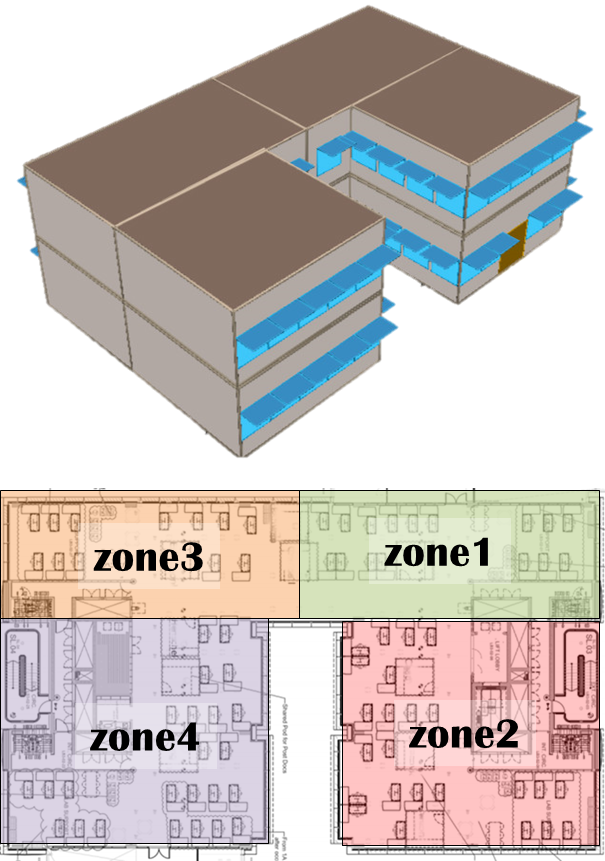
\includegraphics[width=0.9\columnwidth]{./images/zonedivided.png}
  \caption{The simulated Open Office looked like test-bed laboratory}\label{fig:simdesign}
\end{figure}


We demonstrate the potential energy savings for applying an occupancy schedule into controlling the HVAC running time. We used the Masdar Energy Design Guidelines (MEDG)\footnote{Masdar Energy Design Guideline (MEDG) as a baseline for occupancy and thermostat set-points. MEG has been created to specifically serve as a mandatory framework for designing energy efficient buildings in Masdar City.

In the {\em first control case}, we tried to modify occupancy schedules and see the impact on energy consumption for space cooling.  The occupant's schedule  has by default one segment for weekdays and another for weekend. We substituted this schedule by a daily schedule  fed by data from our monitoring system. The potential energy saving difference between the two types of  scheduled  vs. unscheduled occupancy displayed in Figure \ref{fig:engsav}.

\begin{figure}[!ht]
  \centering
 	  	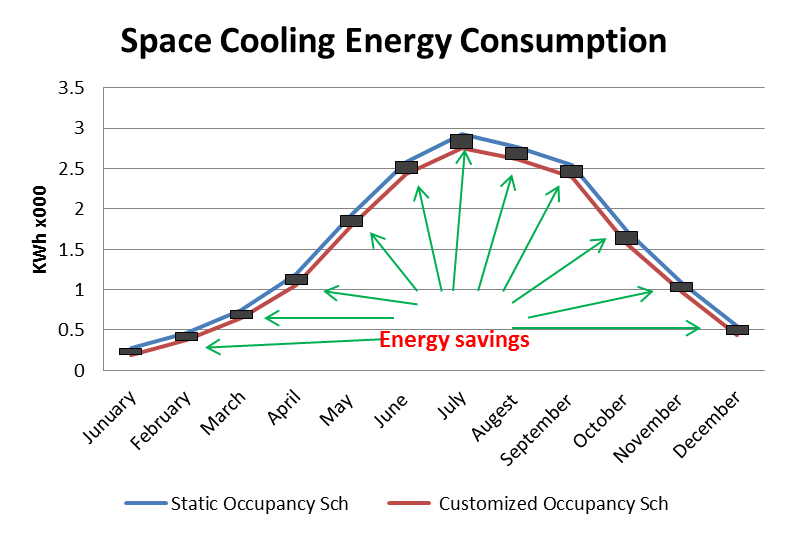
\includegraphics[width=0.9\columnwidth]{./images/energysavings.png}
  \caption{The simulated Open Office looked like test-bed laboratory}\label{fig:engsav}
\end{figure}

In the {\em second control case}, we modified the thermostat set-point schedule and convert it into more dynamic depend on our collected data. The set-point of thermostat is designed to meet the level of comfort, and here we rely on the occupancy density from our sample data to design customized set-point schedule for each day at different time. The results raise the energy consumption savings to 22.1\% as showing in figure  . There are a potential energy savings using customized occupancy/setpoint schedules. Even this small percentage of energy saving in favor of the custom schedule has a significant impact in large buildings. 